\documentclass{article}

% ---------------------------------------------------------------------------
% Representations for the Physical Sciences Workshop, NeurIPS 2026.
% Double-blind review: the "dblblindworkshop" option is used WITHOUT "final"
% and WITHOUT "preprint", so the style file prints "Anonymous Author(s)" and
% adds line numbers. Add "final" only for the camera-ready version.
% ---------------------------------------------------------------------------
\usepackage[dblblindworkshop]{neurips_2026}

\usepackage[utf8]{inputenc} % allow utf-8 input
\usepackage[T1]{fontenc}    % use 8-bit T1 fonts
% Courier for \texttt: the T1-encoded Computer Modern typewriter font is a
% bitmap on many installations, which would put Type 3 fonts in the PDF and
% the submission instructions allow only Type 1 or embedded TrueType.
\renewcommand{\ttdefault}{pcr}
\usepackage[hidelinks]{hyperref}  % hyperlinks, no coloured boxes
% \rf{n} renders the digit n and links it to reference n below.
\newcommand{\rf}[1]{\hyperlink{ref#1}{#1}}
\usepackage{url}            % simple URL typesetting
\usepackage{booktabs}       % professional-quality tables
\usepackage{amsfonts}       % blackboard math symbols
\usepackage{amsmath}        % display math
\usepackage{nicefrac}       % compact symbols for 1/2, etc.
\usepackage{microtype}      % microtypography
\usepackage{xcolor}         % colors
\usepackage{graphicx}       % figures

% \workshoptitle sets the workshop name displayed in the footer.
\workshoptitle{Representations for the Physical Sciences Workshop}

\title{UnLense: Unsupervised Super-Resolution of Gravitational Lensing
Images via a Differentiable Lensing Forward Model}

% Submission is double-blind. The style file suppresses this block and prints
% "Anonymous Author(s)" instead. Real names, affiliations and an
% \begin{ack} ... \end{ack} block go here only in the camera-ready version.
\author{%
  Anonymous Author(s) \\
  Affiliation \\
  Address \\
  \texttt{email} \\
}

\begin{document}

\maketitle

\begin{abstract}
Strong gravitational lensing probes dark matter substructure directly, but
upcoming surveys will find of order $10^{5}$ galaxy-galaxy lenses and follow up
only a small fraction, so the image pairs supervised super-resolution requires
will not exist for most of that population. We present \texttt{UnLense}, which
recovers a lens and a source from a single observation using the forward model
as its only supervision: a differentiable elliptical power-law deflection field,
a measured instrument response and detector binning render any proposed source
into a predicted image, and a $\chi^{2}$ against the observed pixels is the only
training signal. Physics fixes the forward model but not the source
representation, so we measure it on $2{,}000$ held-out Roman-like simulations
across four representations that share one lens, one optimizer and one scorer.
Source error falls monotonically as the number of free source values falls, from
nmse $0.056$ at $3{,}844$ free pixels to $0.017$ at seven analytic parameters, a
ceiling that exists only because these sources are analytic by construction. \texttt{UnLense} recovers seven physical
parameters from the pixels alone at Spearman $+0.59$ to $+0.97$ and reproduces
magnification quantities that never entered the fit. Of structure injected below
the detector pixel scale a median 18 percent returns, and gating the source
prior on local magnification, so that sub-pixel structure is permitted only where
the lens delivers the resolution to constrain it, improves every source-plane
metric on both seeds while the median $\chi^{2}$ shifts by $0.15$ percent.
\end{abstract}

\section{Introduction}

Gravitational lensing bends light from a background galaxy into arcs, rings and
multiple images [\rf{1}]. The deflection depends on the total projected mass and
not on the light, so a lensed image carries information about the small-scale
dark matter substructure that separates competing dark matter models
[\rf{2}, \rf{3}]. Lensing also magnifies, spreading a small patch of the source
across many detector pixels, so super-resolution here is something the geometry
already permits.

Recovering the source means inverting a map that is many-to-one by
construction. The usual machine learning answer is supervised
super-resolution on paired low- and high-resolution images, which has been done
for lensing with a conditional diffusion model trained on matched ground- and
space-based cutouts [\rf{19}]. Those pairs do not exist at the scale required:
that dataset ran to 173 real objects, while Euclid, LSST and Roman are expected
to find of order $10^{5}$ galaxy-galaxy lenses [\rf{4}] and follow-up will reach
a small fraction of them.

An alternative is to use the forward model as the supervision: a candidate lens
and source are ray-traced, convolved with the instrument response, binned onto
detector pixels and compared with the observation, so no high-resolution target
is needed [\rf{5}]. This does not settle what the source should be. The
deflection field is a small parametric family the arcs identify well, while
published choices for the source run from a handful of analytic parameters
[\rf{6}, \rf{7}] through regularized pixel grids [\rf{14}, \rf{15}] to tens of
thousands of free pixels [\rf{8}, \rf{9}], usually by convention rather than by
measurement. Joint lens-and-source inference under a learned score-based prior
has been demonstrated [\rf{16}, \rf{17}]; we propose no new prior but measure
what the choice is worth. We present \texttt{UnLense}, a label-free system that
fits a lens and a
source jointly to each observation, and use it to turn that convention into a
measurement: data, deflection model, instrument model and scoring function are
held fixed while only the source representation varies. We then test whether the
recovered sub-pixel detail is real by injecting structure smaller than a detector
pixel.

\section{Data and methods}
\label{data_and_methods}

\paragraph{Dataset.} Simulated galaxy-galaxy strong lensing images produced with
\texttt{lenstronomy} [\rf{10}] to resemble Roman Space Telescope observations,
$127 \times 127$ detector pixels at $0.10593$ arcsec per pixel, in three dark
matter classes (axion, cold and warm) contributing equally, $10{,}000$ for
training and $2{,}000$ held out, from disjoint splits. Each
system pairs an elliptical power-law deflector with external shear, contributing
no light of its own, with an elliptical S\'ersic source [\rf{6}] and a population
of dark matter subhalos, and stores the noiseless unlensed source and the
simulation parameters, so both can be scored against truth. That stored source is at detector sampling and already
convolved, so no high-resolution target exists in the dataset.

\paragraph{Forward model.} The lens equation is $\boldsymbol{\beta} =
\boldsymbol{\theta} - \boldsymbol{\alpha}(\boldsymbol{\theta})$, with
$\boldsymbol{\alpha}$ the deflection of an elliptical power-law convergence plus
a constant external shear: Einstein radius $\theta_{E}$, radial slope $\gamma$,
two ellipticity and two shear components. This is the standard galaxy-scale mass
model [\rf{11}] and also the family the simulation used, so lens recovery here is
a best case. The closed form of [\rf{11}] calls
\texttt{scipy.special.hyp2f1}, which has no PyTorch equivalent, so we evaluate
the hypergeometric series it sums and reproduce \texttt{lenstronomy}'s
deflection to machine precision. Rays are traced back from each image pixel to the source
plane, the source is sampled there, the sky is convolved with the response and
area-averaged onto detector pixels, in that order, because the optics blur before
the detector integrates (Figure~\ref{fig:pipeline}). The response is measured
rather than assumed: the stored source is the analytic source already convolved
with the true kernel, so the kernel is over-determined and a Wiener-regularized
division in Fourier space stacked over 40 sources recovers it without assuming a
shape (Appendix~\ref{app:psf}).

\paragraph{Objective and initialization.} The objective is $\chi^{2} = \sum_{i}
((m_{i} - d_{i})/\sigma)^{2}$ over a 45 pixel disk holding $6{,}361$ pixels, with
$\sigma$ measured per image from a source-free annulus beyond radius 50. Runs
that train a network replace $\sigma^{2}$ by $\sigma^{2} + (0.02\,m_{i})^{2}$, a
variance floor stating that the model is not trusted to better than two percent
of its own value at any pixel; without it four images in every four hundred carry
half of the batch gradient, because on the brightest arcs a one percent
kernel-shape error is already a $50\sigma$ residual. Every $\chi^{2}$ we report
uses the plain $\sigma$, so the floor cannot flatter a result. No labels, no
high-resolution target and no simulation parameters enter the objective, and
starting values are measured from the image. Six lens parameters are used
because, holding the true source fixed, arc-weighted correlation with the truth
runs $0.799$ for a circular isothermal sphere, $0.966$ for an isothermal
ellipsoid, $0.980$ once the radial slope is freed and $0.996$ for the ellipsoid
with external shear.

\paragraph{Source representations.} The lens model is settled by that
measurement; the source is not, so we compare the five representations of
Table~\ref{tab:reps} under one forward model, optimizer and scorer. Two are free
pixel grids: one at twice detector sampling from a convolutional upsampling
network [\rf{12}, \rf{13}] acting on the observation back-projected into the
source plane, one from the earlier grid pipeline under a total-variation prior.
Two are hybrids in which a fitted S\'ersic carries the wings and the network adds
a bounded residual, decoded either convolutionally or from a pooled vector. The
fifth is the S\'ersic alone. Every network row uses a lens fitted per image and
then frozen, so rows 2--5 share a common lens.

\begin{figure}[t]
  \centering
  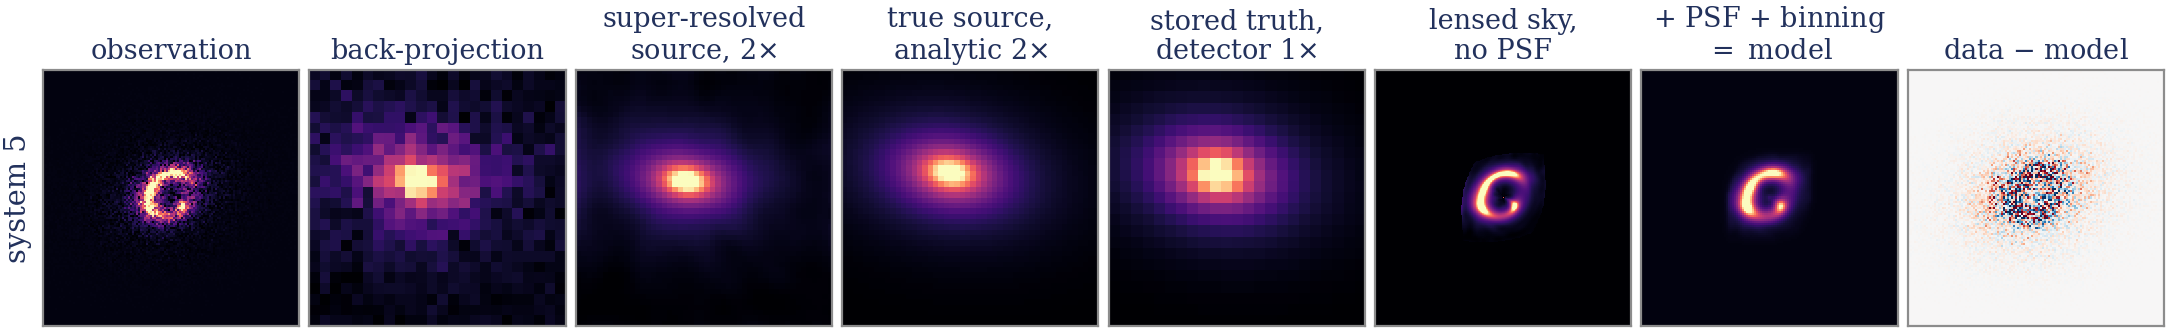
\includegraphics[width=\linewidth]{figs/fig1_pipeline.png}
  \caption{\texttt{UnLense} end to end. The observation is back-projected into
  the source plane, the network returns a source twice as finely sampled as the
  detector, and that source is re-lensed, convolved and binned to close the
  $\chi^{2}$ against the same pixels. The only stored truth is at detector
  sampling and already convolved, so the analytic re-render is for the eye only.}
  \label{fig:pipeline}
\end{figure}

\section{Results}
\label{results}

\paragraph{Parameter and source recovery.} On $2{,}000$ held-out images the
seven simulation parameters are recovered at Spearman rank correlation $+0.973$
($\theta_{E}$), $+0.956$ (S\'ersic index), $+0.947$ (half-light radius), $+0.925$
(source offset), $+0.813$ (lens ellipticity), $+0.645$ (external shear) and
$+0.590$ (radial slope); none was available to the fit. Rank correlation is
insensitive to a monotone bias, so median absolute errors accompany it in
Appendix~\ref{app:params}. The recovered
source matches the stored truth at correlation $0.992$, size ratio $1.061$ and
nmse $0.017$, against a size ratio of $10.6$ to $12.8$ for the earlier grid
pipeline on these data.

\paragraph{Validation on quantities never fit.} Magnification is derived from the
recovered lens and enters no objective. Total magnification is $5.83$ against a
true $5.89$, the tangential critical curve is recovered to a radial root mean
square error of $0.56$ detector pixels, and its azimuthal swing is $0.512$
against $0.554$ arcsec (Figure~\ref{fig:validation}). A circular lens gives a
swing of exactly zero, so recovering it shows the four shape parameters were
recovered jointly, not in magnitude alone.

\paragraph{What $\chi^{2}$ can reach here.} $\chi^{2}/\mathrm{dof}$ settles near
$3{,}600$, not $1$, because the data contain subhalo substructure no smooth model
describes: the \emph{true} source through the \emph{true} lens gives a median of
$6{,}492$ on 500 images, and a fitted smooth source can score below even that.
The residual grows with brightness, $2{,}312$, $5{,}514$ and $40{,}025$ across
three signal-to-noise bins, which marks it as a systematic.

\begin{table}[t]
  \caption{Five source representations scored on the same $2{,}000$ validation
  images against the stored source, convolution matched. ``Data per value'' uses
  the $3{,}878$ pixels above $3\sigma$ in the fit disk. Rows 2--5 are the
  controlled comparison, identical in lens, data, optimizer and scorer; row 1 is
  the earlier pipeline, which also used a fixed circular lens and a
  total-variation prior, so it bounds rather than isolates the cost of a free
  field.}
  \label{tab:reps}
  \centering
  \footnotesize
  \begin{tabular}{lrrccc}
    \toprule
    source representation & free values & data/value & corr & size ratio & nmse \\
    \midrule
    free field, $254^{2}$, circular lens, TV prior & 64,516 & 0.06 & -- & 10.6--12.8 & -- \\
    free field, $62^{2}$, convolutional network & 3,844 & 1.01 & 0.971 & 1.141 & 0.0560 \\
    S\'ersic $+$ $48^{2}$ residual, same network & 7 + 2,304 & 1.68 & 0.983 & 1.048 & 0.0336 \\
    S\'ersic $+$ $32^{2}$ correction, pooled vector & 7 + 1,024 & 3.76 & 0.985 & 1.026 & 0.0297 \\
    S\'ersic only, 7 values & 7 & 554 & \textbf{0.992} & 1.061 & \textbf{0.0166} \\
    \bottomrule
  \end{tabular}
\end{table}

\paragraph{Which source representation the data support.} The table is monotone:
across nearly three orders of magnitude in the number of free source values,
source error falls as that number falls across rows 2--5, which differ in nothing
else. Row 1
sits outside that set: its $254^{2}$ field is underdetermined seventeenfold and
inflates the source tenfold at every prior strength across a hundredfold sweep,
but it also used a fixed circular lens, worth $0.799$ against $0.996$ in
arc-weighted correlation at fixed true source, so part of the inflation is the
lens and not the free values. The two
overdetermined hybrids do not escape it either, at nmse $0.0297$ and $0.0336$,
on different analytic bases, only one improving on its own
(Appendix~\ref{app:extra}). The last row is a ceiling only because these sources
are S\'ersic profiles by construction, so the analytic prior is exactly correct;
the table constrains this dataset, not learned source models in general. On real galaxies, where no analytic family is
correct, a learned source is the only route left, and how many values it may
carry is set by the roughly $3{,}878$ informative pixels an image supplies.

\paragraph{Is the recovered sub-pixel detail real?} Reconstructing on a grid
finer than the detector is meaningful only if the lens supplies the extra
sampling: median tangential stretch is $2.86$ against a radial $0.98$, and the
networks request $2.0$ times. Warrant is not evidence, so we plant a Gaussian
clump of $0.08$ arcsec full width at half maximum, $0.76$ detector pixels, at 15
percent of the source peak, and reconstruct with and without it under one noise
realization, so noise and smooth source cancel in the difference.
Over $2{,}400$ injections across 60 images, none seen during training, a median
18 percent of the injected contrast returns, rising with photon count at partial
rank correlation $+0.33$
(Figure~\ref{fig:validation}A). It does not rise with local magnification, at
$-0.21$, but that comparison is weak by construction: the clump amplitude is
fixed against the \emph{global} source peak, so its local contrast grows with
source-plane radius (Appendix~\ref{app:extra}).

\paragraph{Building magnification into the prior does pay.} A structural gate
applies a sigmoid in $\log \mu$ to the network output before the forward model,
permitting sub-pixel structure only where the lens delivered the resolution to
constrain it. Against a control identical in every other respect it improves
every source-plane metric on both seeds, taking nmse from $0.0336$ and $0.0331$
to $0.0321$ and $0.0321$, two to three times the seed-to-seed spread within the
control (Appendix~\ref{app:gate}). Data fidelity is essentially
unchanged, the median $\chi^{2}/\mathrm{dof}$ moving from $4{,}005$ to $4{,}011$,
$0.15$ percent, while per image the gated model has the lower $\chi^{2}$ on 68
percent of the $2{,}000$ images (Wilcoxon $p = 4 \times 10^{-30}$,
Figure~\ref{fig:validation}B). Weighting the correction penalty by magnification
instead of gating moves nmse from $0.0302$ to $0.0297$, the same way.

\begin{figure}[t]
  \centering
  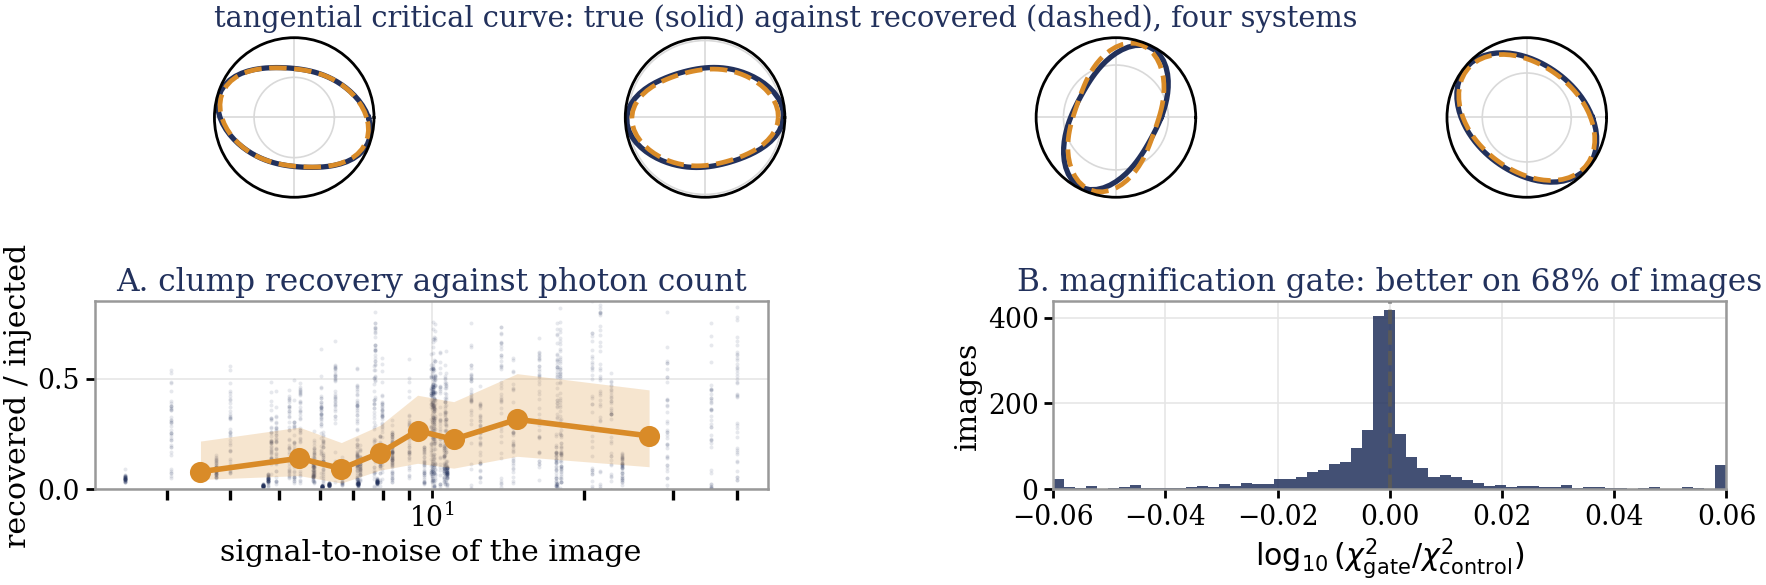
\includegraphics[width=3.75in]{figs/fig2_validation.png}
  \caption{Top, the tangential critical curve of the recovered lens against the
  truth for four systems, none of which entered the fit. A, recovered over
  injected clump contrast against photon count. B, per-image $\chi^{2}$ of the
  gated model relative to its control.}
  \label{fig:validation}
\end{figure}

\paragraph{Amortized inference as an initializer.} A single network forward pass
costs milliseconds against $0.94$ s for a cold per-image fit and matches it on
Einstein radius ($+0.974$) and half-light radius ($+0.978$), but fails on
ellipticity, at $+0.569$ against $+0.776$: a conditional-mean shrinkage of a
spin-2 quantity rather than a misorientation, with median phase error $9$ degrees
while the modulus is shrunk to $0.63$ of the truth, flat across phase-error bins
(Appendix~\ref{app:extra}). We therefore
initialize the fit with the network rather than replace it: with identical bounds
and tolerances the warm fit reaches $\chi^{2}/\mathrm{dof}$
$3{,}571$ in a median 136 model evaluations and $0.41$ s in one stage, against
$3{,}649$ in 475 and $0.94$ s across four stages from cold, improving rank
correlation on all seven parameters.

\section{Limitations and outlook}
\label{limitations}

Transfer outside the fitted lens family is untested. We report point estimates and no
posterior, the largest gap and the one our results point at most directly, since
the modulus shrinkage above is a bias a density head would report as a width.
Magnification is derived from the recovered lens rather than measured
independently, and all data are simulated from one instrument, so nothing here
has met real galaxy morphology or a real point spread function.

Three directions follow. A density head over the fourteen parameters would
report that shrinkage as a width. Real galaxy morphology, from a catalog or from
a learned generative prior, would lift the ceiling of the last table row.
Diffusion models have been applied here both as a conditional low- to
high-resolution map [\rf{19}] and as a source prior inside a forward model
[\rf{16}, \rf{17}, \rf{18}]; only the second needs no pairs, and our gate
result suggests modulating its strength by local magnification. Finally, the lens is achromatic and both bands are present,
so a two-band fit would constrain one lens with twice the data.

\section*{References}

{
\small

\hypertarget{ref1}{[1]} Bartelmann, M.\ (2010) Gravitational lensing. {\it Classical and Quantum
Gravity} {\bf 27}(23):233001.

\hypertarget{ref2}{[2]} Vegetti, S.\ \& Koopmans, L.V.E.\ (2009) Bayesian strong gravitational-lens
modelling on adaptive grids. {\it Monthly Notices of the Royal Astronomical
Society} {\bf 392}:945.

\hypertarget{ref3}{[3]} Heinze, F.M., Despali, G.\ \& Klessen, R.S.\ (2023) Not all subhaloes are
created equal. {\it Monthly Notices of the Royal Astronomical Society}
{\bf 527}(4):11996.

\hypertarget{ref4}{[4]} Collett, T.E.\ (2015) The population of galaxy-galaxy strong lenses in
forthcoming optical imaging surveys. {\it The Astrophysical Journal}
{\bf 811}:20.

\hypertarget{ref5}{[5]} Shankar, A., Toomey, M.W.\ \& Gleyzer, S.\ (2024) Unsupervised
physics-informed super-resolution of strong lensing images for sparse datasets.
{\it Machine Learning and the Physical Sciences workshop, NeurIPS}.

\hypertarget{ref6}{[6]} Cardone, V.\ (2003) The lensing properties of the S\'ersic model.
{\it Astronomy and Astrophysics} {\bf 415}:11.

\hypertarget{ref7}{[7]} Hezaveh, Y.D., Perreault Levasseur, L.\ \& Marshall, P.J.\ (2017) Fast
automated analysis of strong gravitational lenses with convolutional neural
networks. {\it Nature} {\bf 548}:555.

\hypertarget{ref8}{[8]} Morningstar, W.R.\ et al.\ (2019) Data-driven reconstruction of
gravitationally lensed galaxies using recurrent inference machines.
{\it The Astrophysical Journal} {\bf 883}:14.

\hypertarget{ref9}{[9]} Adam, A., Perreault Levasseur, L., Hezaveh, Y.\ \& Welling, M.\ (2022)
Pixelated reconstruction of foreground density and background surface brightness
in gravitational lensing systems using recurrent inference machines.
{\it The Astrophysical Journal} {\bf 925}:124.

\hypertarget{ref10}{[10]} Birrer, S.\ \& Amara, A.\ (2018) lenstronomy: multi-purpose gravitational
lens modelling software package. {\it Physics of the Dark Universe}
{\bf 22}:189.

\hypertarget{ref11}{[11]} Tessore, N.\ \& Metcalf, R.B.\ (2015) The elliptical power law profile
lens. {\it Astronomy and Astrophysics} {\bf 580}:A79.

\hypertarget{ref12}{[12]} Ledig, C.\ et al.\ (2017) Photo-realistic single image super-resolution
using a generative adversarial network. {\it CVPR}.

\hypertarget{ref13}{[13]} Shi, W.\ et al.\ (2016) Real-time single image and video super-resolution
using an efficient sub-pixel convolutional neural network. {\it CVPR}.

\hypertarget{ref14}{[14]} Suyu, S.H., Marshall, P.J., Hobson, M.P.\ \& Blandford, R.D.\ (2006) A
Bayesian analysis of regularized source inversions in gravitational lensing.
{\it Monthly Notices of the Royal Astronomical Society} {\bf 371}:983.

\hypertarget{ref15}{[15]} Karchev, K., Coogan, A.\ \& Weniger, C.\ (2022) Strong-lensing source
reconstruction with variationally optimized Gaussian processes.
{\it Monthly Notices of the Royal Astronomical Society} {\bf 512}:661.

\hypertarget{ref16}{[16]} Adam, A., Coogan, A., Malkin, N., Legin, R., Perreault
Levasseur, L., Hezaveh, Y.\ \& Bengio, Y.\ (2022) Posterior samples of source
galaxies in strong gravitational lenses with score-based priors. {\it Machine
Learning and the Physical Sciences workshop, NeurIPS}. arXiv:2211.03812.

\hypertarget{ref17}{[17]} Barco, G.M., Legin, R., Stone, C., Hezaveh, Y.\ \&
Perreault-Levasseur, L.\ (2025) Blind strong gravitational lensing inversion:
joint inference of source and lens mass with score-based models. {\it Workshop on
Machine Learning for Astrophysics, ICML}. arXiv:2511.04792.

\hypertarget{ref18}{[18]} Payeur, G., Perreault-Levasseur, L., Barco, G.M.\ \&
Hezaveh, Y.\ (2026) Strong gravitational lensing posterior sampling in
pixel-space using diffusion models and recurrent inference machines.
arXiv:2607.19459.

\hypertarget{ref19}{[19]} Reddy, P., Toomey, M.W., Parul, H.\ \& Gleyzer, S.\
(2024) DiffLense: a conditional diffusion model for super-resolution of
gravitational lensing data. {\it Machine Learning: Science and Technology}
{\bf 5}(3):035076.

}

%%%%%%%%%%%%%%%%%%%%%%%%%%%%%%%%%%%%%%%%%%%%%%%%%%%%%%%%%%%%

\appendix

\section{Further reconstructions}
\label{app:pipeline_extra}

The forward chain drawn in Figure~\ref{fig:pipeline} and
Figure~\ref{fig:pipeline_extra} is the project's own renderer run under NumPy
from the frozen lens fit and the stored source map; it reproduces the PyTorch
predictions used in every metric to $0.4$ percent rms of the image peak.

\begin{figure}[h]
  \centering
  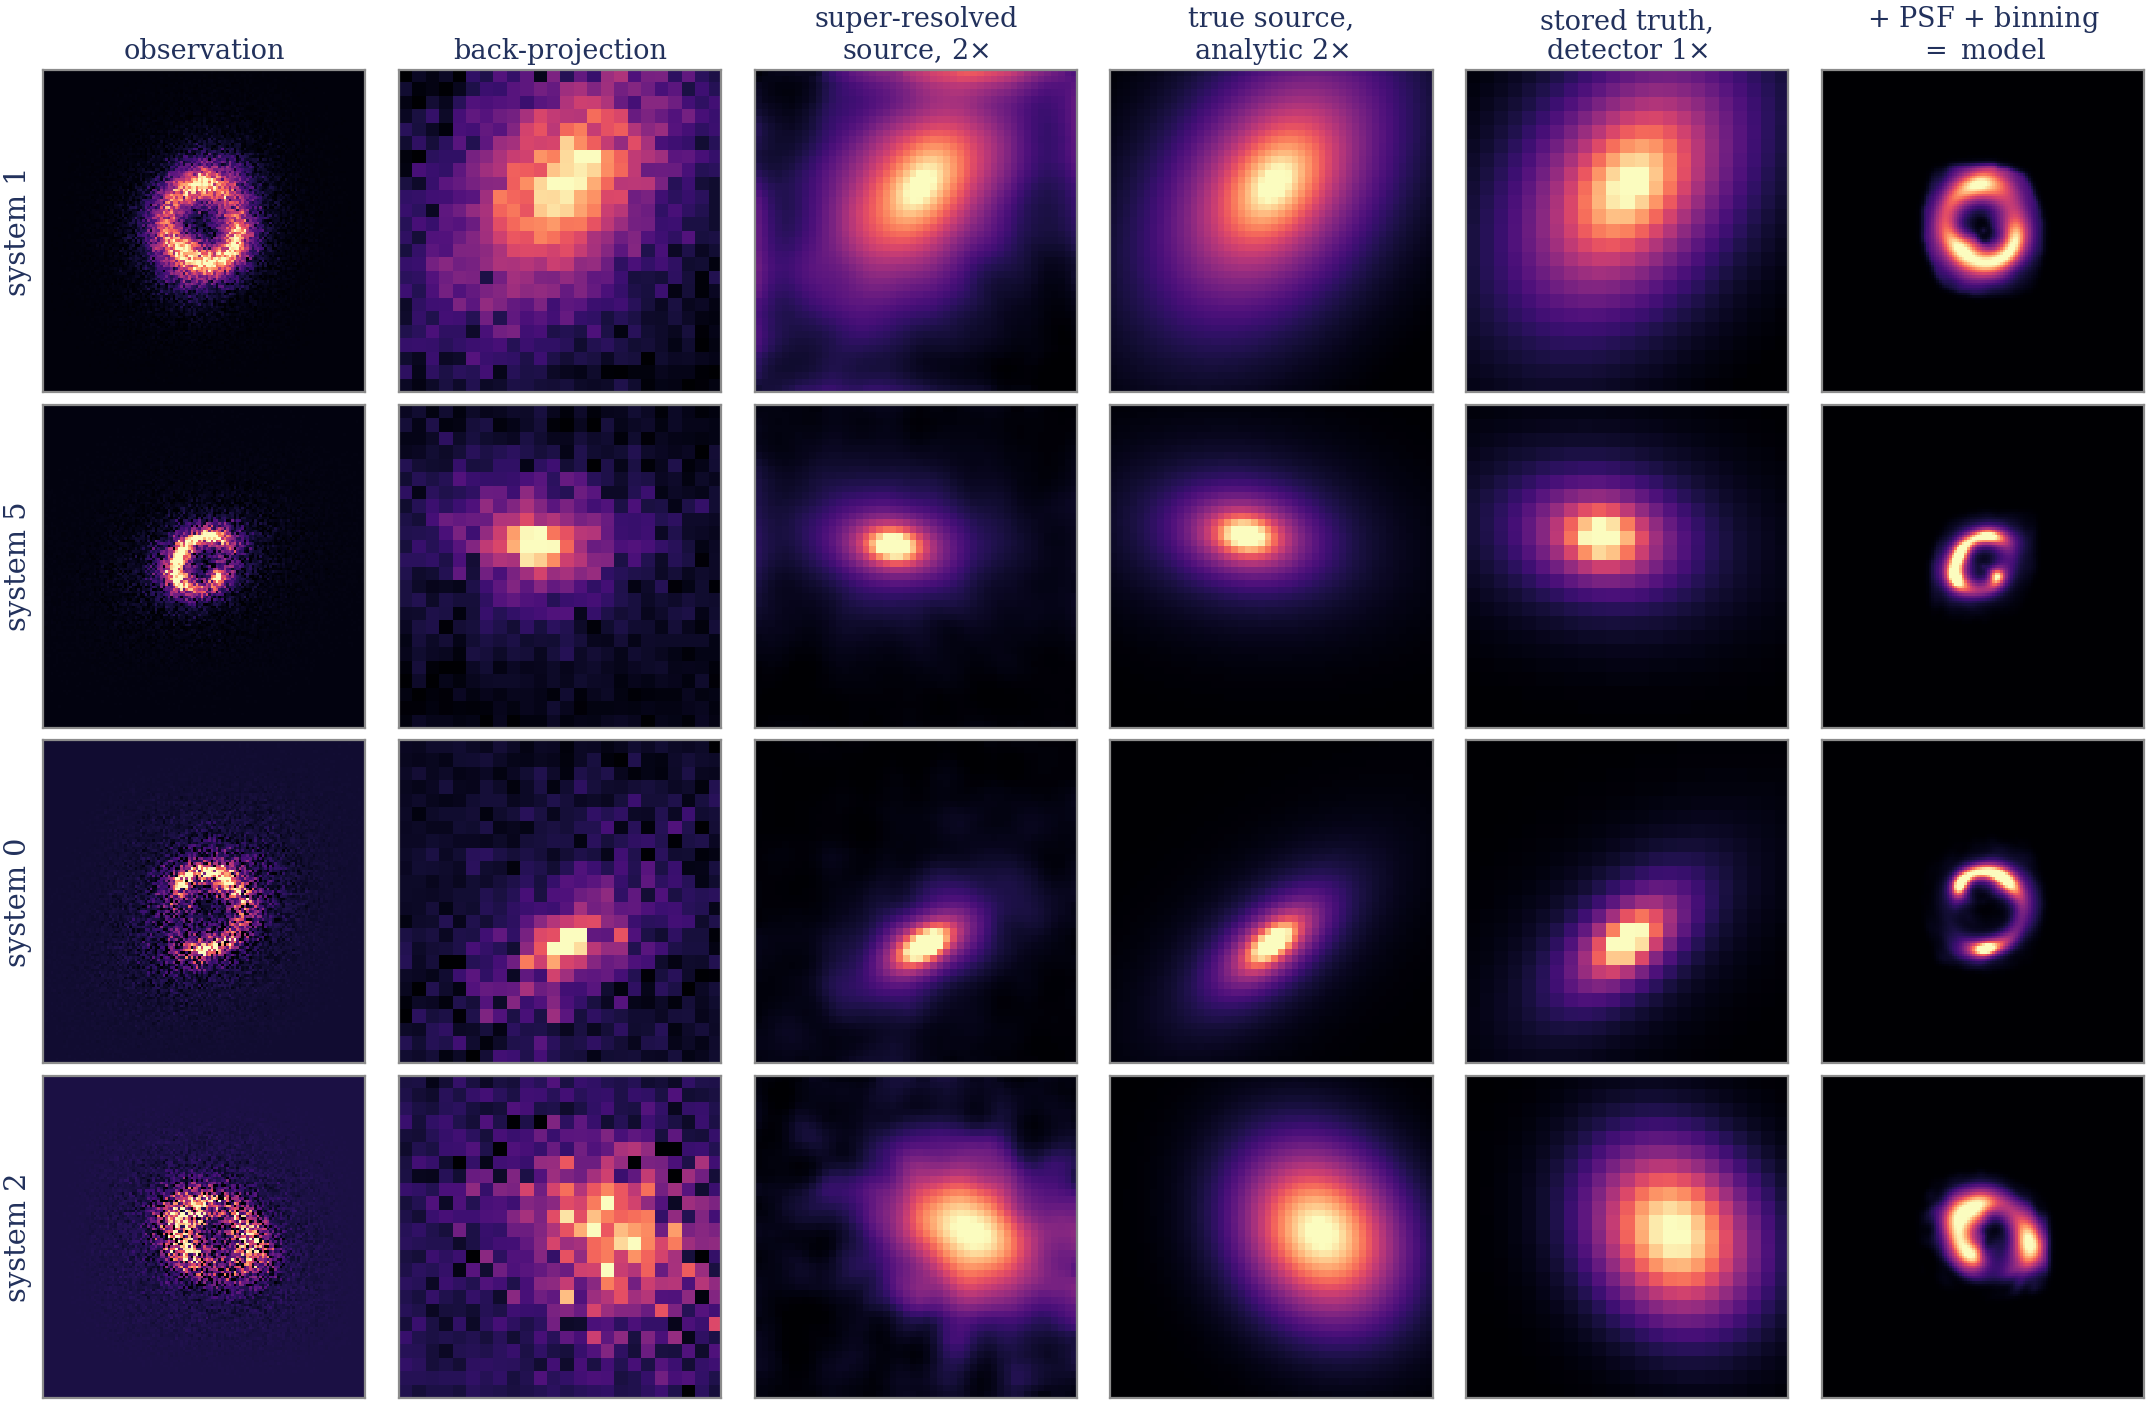
\includegraphics[width=\linewidth]{figs/figA_pipeline_extra.png}
  \caption{Four further validation systems through the pipeline of
  Figure~\ref{fig:pipeline}, spanning the signal-to-noise range of the
  validation set. Panels and scaling follow that figure.}
  \label{fig:pipeline_extra}
\end{figure}

\section{Full parameter recovery}
\label{app:params}

Per-image bounded nonlinear least squares (trust-region reflective rather than
plain Levenberg-Marquardt, since several parameters carry hard bounds),
initialized from the amortized network, $n = 2{,}000$ across the three dark
matter classes.

\begin{table}[h]
  \centering
  \small
  \begin{tabular}{lrrrrr}
    \toprule
    parameter & fit median & true median & median abs.\ err & p90 abs.\ err & Spearman \\
    \midrule
    $\theta_{E}$ (arcsec) & 1.300 & 1.310 & 0.047 & 0.102 & $+0.973$ \\
    $\beta$ (arcsec) & 0.287 & 0.306 & 0.030 & 0.089 & $+0.925$ \\
    $R_{\mathrm{sersic}}$ (arcsec) & 0.514 & 0.489 & 0.039 & 0.180 & $+0.947$ \\
    $n_{\mathrm{sersic}}$ & 1.183 & 1.003 & 0.174 & 0.901 & $+0.956$ \\
    slope $\gamma$ & 2.015 & 2.050 & 0.068 & 0.233 & $+0.590$ \\
    lens $|e|$ & 0.203 & 0.219 & 0.031 & 0.107 & $+0.813$ \\
    shear $|g|$ & 0.048 & 0.033 & 0.014 & 0.052 & $+0.645$ \\
    \bottomrule
  \end{tabular}
\end{table}

Source plane, scored against the stored source with the model convolved first:
correlation $0.9918$, size ratio $1.061$, centroid error $0.353$ pixels, peak
ratio $0.863$, nmse $0.0166$. Median $\chi^{2}/\mathrm{dof}$ is $3{,}571$, with
the plain background $\sigma$ over the $6{,}361$ pixel fit disk divided by
$6{,}361 - 14$ for the fourteen free parameters. The radial slope is the least
constrained parameter and sits close to isothermal.

\section{Instrument response}
\label{app:psf}

The stored unlensed array is the analytic source already convolved with the true
kernel, so in Fourier space the kernel is the ratio of the two transforms. Naive
division amplifies noise wherever the source transform is small, so we use the
Wiener form, replacing $1/\hat{s}$ by
$\bar{\hat{s}}/(|\hat{s}|^{2} + \lambda)$, and stack over 40 sources. This
assumes nothing about the kernel's shape, which is the point: a parametric sweep
over Gaussian widths bottoms out at a residual nmse of a few times $10^{-3}$
rather than at zero, so the true kernel is not Gaussian, and on arcs reaching
peak-to-background ratios of $10^{3}$ to $10^{4}$ a one percent shape error is a
$50\sigma$ per-pixel residual. The recovered kernel carries $22$ percent of its
flux beyond $0.25$ arcsec against $13$ percent for the Gaussian that best fits
the same kernel in least squares.

\section{Resolution is not a rendering choice}
\label{app:resolution}

The parametric source is continuous and can be sampled on any grid. Scored
against the stored source rendered on the same grid, $n = 2{,}000$:

\begin{table}[h]
  \centering
  \small
  \begin{tabular}{lrrrr}
    \toprule
    factor & scale (arcsec/px) & corr & nmse & size ratio \\
    \midrule
    $1\times$ & 0.1059 & 0.9843 & 0.0309 & 0.950 \\
    $2\times$ & 0.0530 & 0.9835 & 0.0326 & 0.928 \\
    $4\times$ & 0.0265 & 0.9832 & 0.0335 & 0.912 \\
    $8\times$ & 0.0132 & 0.9830 & 0.0336 & 0.906 \\
    \bottomrule
  \end{tabular}
\end{table}

Correlation moves by $0.0013$ across an eightfold range, so the sampling of the
render is not what limits the reconstruction.

\section{Magnification-adaptive regularization}
\label{app:gate}

Both variants make the source prior depend on the local magnification of the
recovered lens. The weaker one weights the curvature penalty on the $32^{2}$
correction by $\mu^{1/2}$; it concentrates the correction where the lens
magnifies, at rank correlation $+0.50$ between correction amplitude and
$\log \mu$ against $+0.32$ for a uniform control, and moves source nmse from
$0.0302$ to $0.0297$. The stronger one gates the $48^{2}$ representation, passing
the network output through a sigmoid in $\log \mu$ before the forward model.

\begin{table}[h]
  \centering
  \small
  \begin{tabular}{lrcccc}
    \toprule
    run & epochs & corr & size ratio & peak ratio & nmse \\
    \midrule
    control, seed 0 & 100 & 0.9829 & 1.048 & 0.930 & 0.0336 \\
    control, seed 1 & 50 & 0.9833 & 1.039 & 0.946 & 0.0331 \\
    gate, seed 0 & 100 & 0.9838 & 1.033 & 0.952 & \textbf{0.0321} \\
    gate, seed 1 & 50 & 0.9837 & 1.041 & 0.940 & \textbf{0.0321} \\
    \bottomrule
  \end{tabular}
\end{table}

The two gated runs agree to four decimals in nmse and both sit below both
controls, whose own seed spread is $0.0005$. The gate sits before the likelihood,
so in principle the network can learn its inverse and undo it; the measured
outcome is that it does not, and the constraint survives. The gate does not lower
the median $\chi^{2}/\mathrm{dof}$, which is $4{,}011$ against the control's
$4{,}005$, while the paired per-image comparison favors it on 68 percent of the
same images. The two statistics disagree because they measure different things:
the medians come from two separate distributions, whereas the paired test sees a
skewed difference, a small gain on most images against a larger loss on a
minority.

\section{Additional detail}
\label{app:extra}

\paragraph{The two hybrid rows.} They are not added to the same base. The
$48^{2}$ residual sits on the per-image S\'ersic and takes source nmse from
$0.0166$ to $0.0336$. The $32^{2}$ correction sits on a S\'ersic the network
predicts itself and improves that base from $0.0311$ to $0.0297$; the base is
already worse than the fitted one, which is why the corrected row still lands
above the analytic row of Table~\ref{tab:reps}.

\paragraph{Informative pixels.} Across 300 validation images in the three
classes, the fit disk of $6{,}361$ pixels contains a mean of $3{,}878$ pixels
above $3\sigma$ (p10 $3{,}196$, p90 $4{,}545$). This is the denominator of the
``data per value'' column in Table~\ref{tab:reps}.

\paragraph{Spin-2 shrinkage.} Modulus ratio by phase-error bin for the amortized
network: $0.63$, $0.64$, $0.61$ and $0.57$ across $0$ to $5$, $5$ to $15$, $15$
to $30$ and $30$ to $90$ degrees, with counts $611$, $726$, $387$ and $276$. The
per-image fit shows a median phase error of $3.3$ degrees and a modulus ratio of
$0.90$ on the same images.

\paragraph{Injection detail.} Recovered clump contrast correlates at $+0.52$ with
the clump's source-plane radius, the strongest single predictor in the set,
because the amplitude is fixed against the global source peak and not the local
one. Whole-source reconstruction error falls from
$0.34$ in the $\mu = 1$ to $2$ bin to $0.018$ at $\mu = 8$ to $16$, on per-bin
image counts of $51$, $60$, $60$, $58$ and $24$; that trend is confounded with
brightness, which is what the paired injection controls for. The clump is fixed
at 15 percent of the global source peak wherever it lands, so the absolute
contrast scale is arbitrary and only relative trends are interpretable.

\paragraph{Reproduction.} Code and exact commands will be released through an
anonymized repository at review time. All runs use a single seed unless stated
otherwise, and the $\chi^{2}/\mathrm{dof}$ convention is the one given in
Appendix~\ref{app:params}.

%%%%%%%%%%%%%%%%%%%%%%%%%%%%%%%%%%%%%%%%%%%%%%%%%%%%%%%%%%%%

\end{document}
